\documentclass[10pt,mathserif]{beamer}

\usepackage{graphicx,amsmath,amssymb,tikz,psfrag,subfigure,bm}

\input defs.tex

%% formatting

\mode<presentation>
{
\usetheme{default}
}
\setbeamertemplate{navigation symbols}{}
\usecolortheme[rgb={0,0,0}]{structure}
\setbeamertemplate{itemize subitem}{--}
\setbeamertemplate{frametitle} {
	\begin{center}
	  {\large\bf \insertframetitle}
	\end{center}
}

\AtBeginSection[] 
{ 
	\begin{frame}<beamer> 
		\frametitle{Outline} 
		\tableofcontents[currentsection,currentsubsection] 
	\end{frame} 
} 

%% begin presentation

\title{\large \bfseries Clustering}

\author{Jiali Lin\\[3ex]
Virginia Tech}

\date{\today}

\begin{document}

\frame{
\thispagestyle{empty}
\titlepage
}

\section{Introduction}
\begin{frame}{Introduction}
\begin{columns}
\column{0.5\textwidth}
\textbf{Similarity-based clustering} 
\begin{itemize}
    \item Input: an $N\times N$ \textbf{dissimilarity matrix}.
    \item Output: \textbf{flat clustering}, where we partition the objects into disjoint sets.
    \item Sensitive to the initial conditions and requires some model selection method for $K$.
\end{itemize}

\column{0.5\textwidth}
\textbf{Feature-based clustering} 
\begin{itemize}
    \item Input: an $N \times D$ feature matrix.
    \item Output: \textbf{hierarchical clustering}, where we create a nested tree of partitions.
    \item Most are deterministic and do not require the specification of $K$.
\end{itemize}
\end{columns}
\end{frame}

\begin{frame}{Clustering Evaluation: Rand Index}
The validation of clustering structures is the most difficult.
\begin{itemize}
    \item The number of assumed clusters may be different.
    \item No true cluster labels.
\end{itemize}    
\bigskip
Rand index computes following for all pairs of data points 
\begin{equation*}\small
    R = \frac{TP+TN}{TP +FP +FN +TN}
\end{equation*}
\begin{itemize}
    \item \textcolor{red}{False positive (FP)}: target splits but algorithm clusters.
    \item \textcolor{red}{False negative (FN)}: target clusters but algorithm splits.
    \item \textcolor{green}{True positive (TP)}: algorithm and target both cluster together.
    \item \textcolor{green}{True negative (TN)}: algorithm and target both split apart.
\end{itemize}

\begin{figure}[h]
\centering
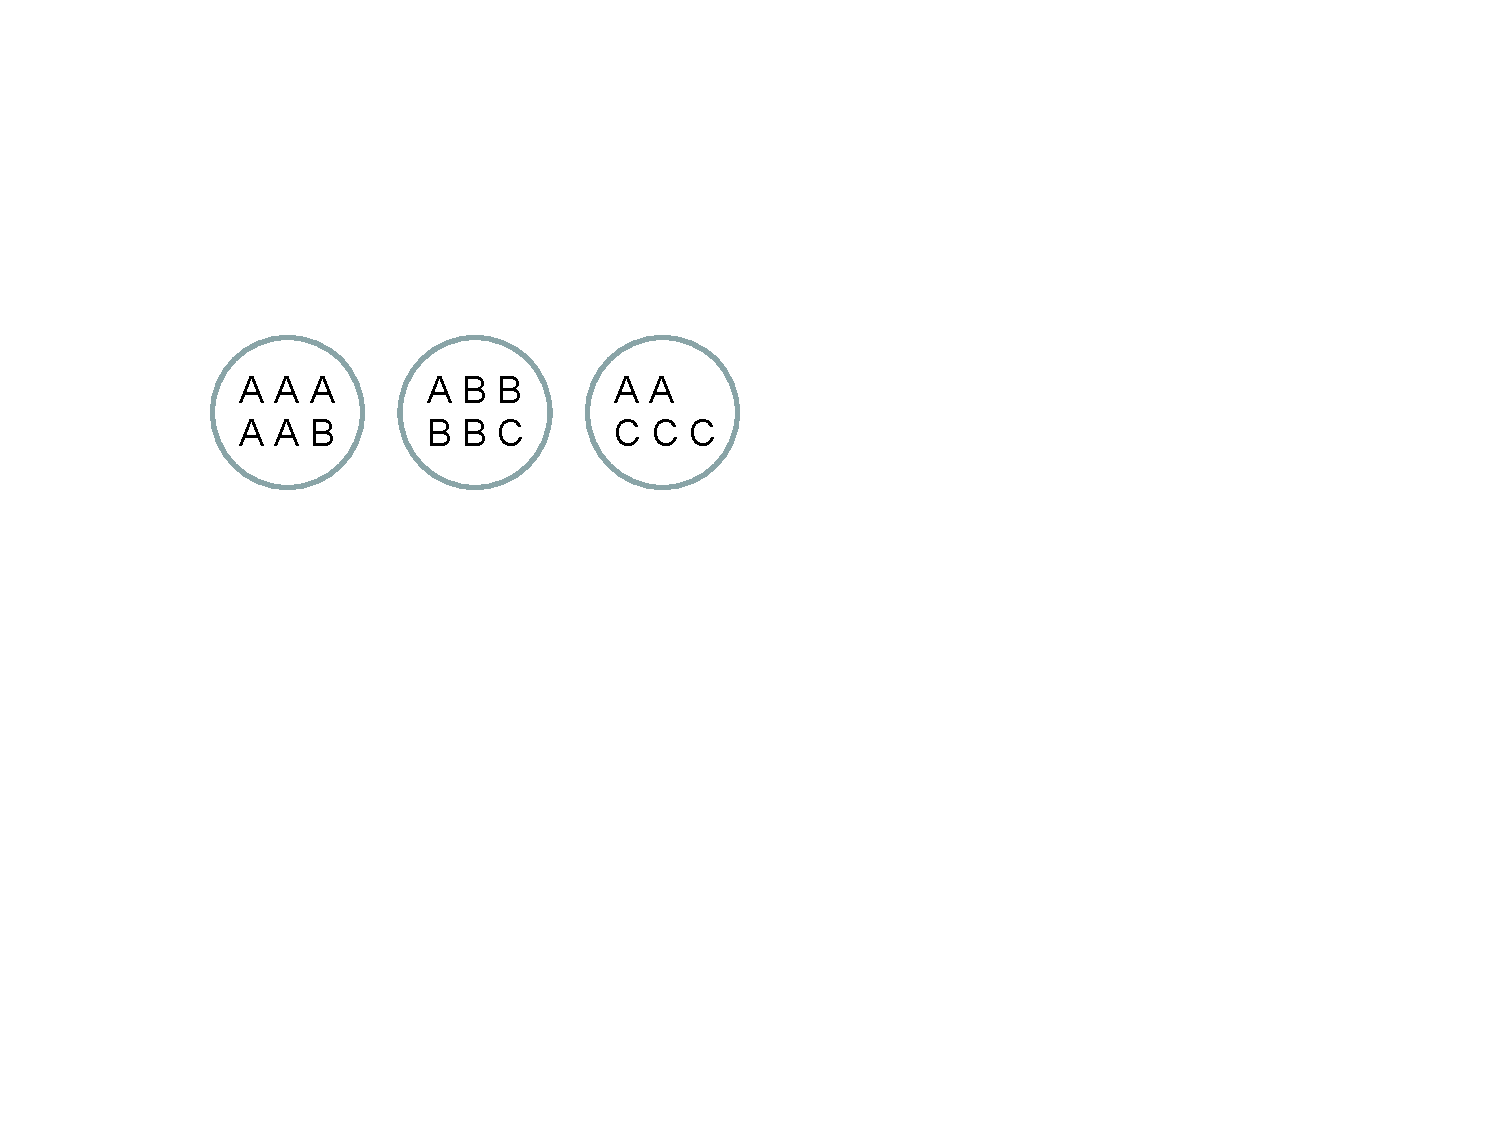
\includegraphics[width=0.4\textwidth]{clusterPurity}
\caption{Circles are proposed clusters, letters are true cluster labels. Invariant to label choices, and takes time linear in $N$. }
\end{figure} 
\end{frame}

\section{Finite mixture models}
\begin{frame}{Finite mixture models}
Traditional representation of a finite mixture model
\begin{equation*}
    \begin{split}
    p(\bm{x}_i|z_i = k, \bm{\theta}) & = p(\bm{x}_i|\bm{\theta_k})\\
    p(z_i = k|\bm{\pi}) & = \pi_k\\
    p(\bm{\pi}|\alpha) & = \text{Dir}(\bm{\pi}|(\alpha/K)\bm{1}_K)
    \end{split}
\end{equation*}

\begin{figure}[h]
\centering
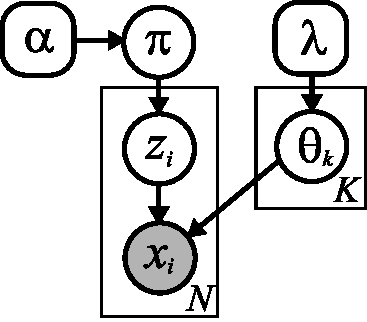
\includegraphics[width=0.25\textwidth]{sudderth-finiteMixIndGraph}
%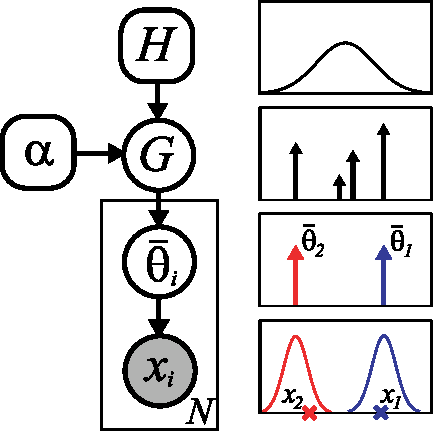
\includegraphics[width=0.75\textwidth]{sudderth-finiteMixDistGraphExampleData}
%\caption{}
\end{figure}

\begin{itemize}
    \item The form of $p(\bm{\theta}_k|\lambda)$ is chosen to be conjugate to $p(\bm{x}_i|\bm{\theta}_k)$. 
    \item We can write $p(\bm{x}_i|\bm{\theta}_k)$ as $\bm{x}_i \sim F(\bm{\theta}_{z_i})$, where $F$ is the observation distribution. 
    \item We can write $\bm{\theta}_k \sim H(\lambda)$, where $H$ is the prior.
\end{itemize}
\end{frame}

\begin{frame}{Another representation}
Consider
\begin{equation*}
        G(\bm{\theta}) = \sum_{k= 1}^K \pi_k\delta_{\bm{\theta}_k} (\bm{\theta})
\end{equation*}
\begin{figure}[h]
\centering
%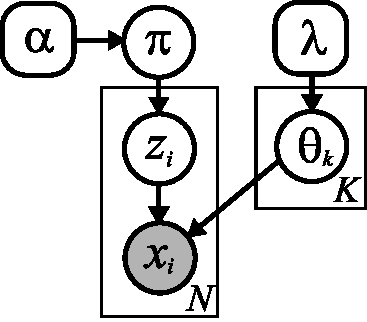
\includegraphics[width=0.25\textwidth]{sudderth-finiteMixIndGraph}
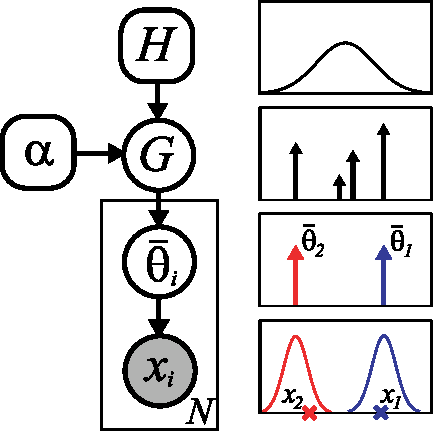
\includegraphics[width=0.25\textwidth]{sudderth-finiteMixDistGraphExampleData}
\caption{Here $\bar{\bm{\theta}}_i$ is the parameter used to generate observation $\bm{x}_i$; these parameters are sampled from distribution $G$, which has the form.}
\end{figure}

\begin{itemize}
    \item The discrete measure, $G$ is a finite mixture of delta functions, $K$ centered on the cluster parameters $\bm{\theta}_k$. 
    \item The probability that $\bar{\bm{\theta}}_i$ is equal to $\bm{\theta}_k$ is exactly $\pi_k$, the prior probability for that cluster.
\end{itemize}    
\end{frame}


\begin{frame}{Generative model}
\begin{itemize}
    \item Finite Gaussian mixture model ($K=2$ clusters)
    \begin{equation*}
        \begin{split}
            z_n & \overset{iid}{\sim} \text{Categorical}(\rho_1,\rho_2)\\
            \bm{x_n} & \overset{indep}{\sim} N(\bm{\mu}_{z_n},\bm{\Sigma})
        \end{split}
    \end{equation*}
    \item Don't know $\mu_1,\mu_2$
    \begin{equation*}
        \bm{\mu_k} \overset{iid}{\sim} N(\bm{\mu}_0,\bm{\Sigma}_0)
    \end{equation*}
    \item Don't know $\rho_1,\rho_2$
    \begin{equation*}
        \begin{split}
            \rho_1 & \sim\text{Beta}(a_1,a_2)\\
            \rho_2 & = 1 - \rho_1
        \end{split}
    \end{equation*}
    \item \textbf{Inference goal}: assignments of data points to clusters, cluster parameters
\end{itemize}    
\end{frame}

\begin{frame}{Generative model}
\begin{itemize}
    \item Finite Gaussian mixture model ($K$ clusters)
    \begin{equation*}
        \begin{split}
            \bm{\rho}_{1:K} & \sim \text{Dirichlet}(a_{1:K})\\
            \bm{\mu}_k & \overset{iid}{\sim} N(\bm{\mu}_0,\bm{\Sigma}_0)\\
            z_n & \overset{iid}{\sim} \text{Categorical}(\bm{\rho}_{1:K})\\
            \bm{x}_n & \overset{indep}{\sim} N(\bm{\mu}_{z_n},\bm{\Sigma})
        \end{split}
    \end{equation*}
\end{itemize}    

\end{frame}

\begin{frame}{What if $K \rightarrow \infty$}
\begin{itemize}
    \item Now, we will always (with probability one) get exactly $K$ clusters.
    \item  Want more flexible model: generate a variable number of clusters.
    \item The more data we generate, the more likely to see a new cluster.
    \item \textbf{Solutions:} replace the discrete distribution $G$ with a \textbf{random probability measure}.
    \item Recall
    \begin{equation*}
        G(\bm{\theta}) = \sum_{k= 1}^K \pi_k\delta_{\bm{\theta}_k} (\bm{\theta})
    \end{equation*}
    \textbf{$\bm{\theta}_i$ can take on the same value $\bm{\theta}_k$ for some $k$}.
\end{itemize}    
\end{frame}

\section{The Dirichlet process}
\begin{frame}{Dirichlet Distribution and Multinomial}
\begin{itemize}
    \item Consider
    \begin{equation*}
        \begin{split}
            (\pi_1,\ldots,\pi_K) & \sim \text{Discrete}(\alpha_1,\ldots,\alpha_K)\\ z|(\pi_1,\ldots,\pi_K) & \sim \text{Discrete}(\pi_1,\ldots,\pi_K)
        \end{split}    
    \end{equation*}
    \item Then
    \begin{equation*}
        \begin{split}
            z & \sim  \text{Discrete}(\frac{\alpha_1}{\sum_i\alpha_i},\ldots, \frac{\alpha_K}{\sum_i\alpha_i})\\
            (\pi_1,\ldots,\pi_K)|z & \sim \text{Discrete}(\alpha_1 +  \delta_1(z),\ldots,\alpha_K + \delta_K(z))
        \end{split}
    \end{equation*}
    where $\delta_i(z) =1$ if $z$ takes on value $i$, $0$ otherwise.
\end{itemize}    
\end{frame}

\begin{frame}{Dirichlet process} 
\begin{itemize}
    \item \textbf{Dirichlet process} is a distribution over probability measures $G: \Theta \rightarrow \mathbb{R}^+$.
    \item Require $G(\theta) \geq 0$ and $\int_\theta G(\theta)d\theta = 1$.
    \item For any finite partition $(T_1,\ldots,T_K)$ of $\Theta$
    \begin{equation*}
        (G(T_1),\ldots,G(T_k))\sim\text{Dir}(\alpha H(T_1),\ldots, \alpha H(T_K )) 
    \end{equation*}
    \item Define: $G \sim \text{DP}(\alpha,H)$, where $\alpha$ is called the \textbf{concentration parameter} and H is called the \textbf{base measure}.
    \item Intuitively, $G$ needs to resemble with the basic distribution $H$.
    \item $\alpha$ determines how closely the histogram of spikes represents $H$.
\end{itemize}    
\end{frame}

\begin{frame}{Some properties of DP}
\begin{itemize}
    \item We are interested in
    \begin{equation*}
        \begin{split}
            p(\theta) & = \int p(\theta|G)p(G)dG \\
            p(G|\theta) & = \frac{p(\theta|G)p(G)}{p(\theta)}
        \end{split}    
    \end{equation*}
    \item Recall \textbf{Dirichlet-multinomial conjugacy}.
    \item If $G\sim\text{DP}(\alpha,H)$, then $p(\bm{\theta}_i\in T_i) = H(T_i)$ and the posterior is
    \begin{equation*}\small
        (G(T_1),\ldots,G(T_k))|\bm{\theta} \sim  \text{Dir}(\alpha H(T_1) + \mathbb{I}(\bm{\theta}\in T_1),\ldots, \alpha H(T_K)+ \mathbb{I}(\bm{\theta}\in T_K))
    \end{equation*}
    \item If we observe multiple samples $\bm{\theta}_i\sim G$
    \begin{equation*}\small
        G|\bm{\theta}_{1:n},\alpha,H \sim \text{DP}(\alpha + n, \frac{\alpha}{\alpha+n}H + \frac{1}{\alpha+n}\sum_{i=1}^n\delta_{\bm{\theta}_i})
    \end{equation*}
\end{itemize}    
\end{frame}

\begin{frame}{Stick-breaking Construction}
\begin{itemize}
    \item Consider a partition $(\bm{\theta}, \bm{X}\backslash\bm{\theta})$ of $\bm{X}$.
    \item We know the the posterior process
    \begin{equation*}\small
        \begin{split}
            (G(\bm{\theta}),G(\bm{X}\backslash\bm{\theta})) & \sim 
            \text{Dir}((\alpha+1)\frac{\alpha H + \delta_{\bm{\theta}}}{\alpha+1}(\bm{\theta}),(\alpha+1)\frac{\alpha H + \delta_{\bm{\theta}}}{\alpha+1}(\bm{X}\backslash\bm{\theta}))\\
            & = \text{Dir}(1,\alpha)
        \end{split}
    \end{equation*}
    \item $G$ has a point mass located at $\bm{\theta}$:
    \begin{equation*}
        G = \beta\delta_{\bm{\theta}} + (1-\beta)G' \quad \text{with} \quad \beta\sim\text{Beta}(1,\alpha)
    \end{equation*}
    \item $G'$ is the (renormalized) probability measure with the point mass removed.
\end{itemize}    
\end{frame}

\begin{frame}{Stick-breaking Construction (cont'd )}
\begin{itemize}
    \item Currently, we have
    \begin{equation*}
        \begin{split}
            G & \sim \text{DP}(\alpha + 1, \frac{\alpha H + \delta_{\bm{\theta}}}{\alpha+1})\\
            G & = \beta\delta_{\bm{\theta}} + (1-\beta)G' \\
            \bm{\theta} & \sim H\\
            \beta & \sim \text{Beta}(1,\alpha)   
        \end{split}
    \end{equation*}
    \item Consider a further partition $(\bm{\theta}, T_1, \ldots, T_K)$ of $\bm{X}$
    \begin{equation*}\small
        \begin{split}
            (G(\bm{\theta}), G(T_1), \ldots, G(T_K))  & =   (\beta,(1-\beta)G'(T_1),\ldots,(1-\beta)G'(T_K))\\ 
            & \sim \text{Dir}(1, \alpha H(T_1),\ldots, \alpha H(T_K))
        \end{split}
    \end{equation*}
    \item The agglomerative/decimative property of Dirichlet implies
    \begin{equation*}\small
        \begin{split}
            (G(T_1),\ldots,G(T_k)) & \sim \text{Dir}(\alpha H(T_1),\ldots, \alpha H(T_K )) \\
            G' & \sim \text{DP}(\alpha,H)
        \end{split}
    \end{equation*}
\end{itemize}    
\end{frame}

\begin{frame}{Stick-breaking Construction (cont'd )}
\begin{itemize}
    \item We have
    \begin{equation*}
        \begin{split}
            G & \sim \text{DP}(\alpha, H)\\
            G & = \beta_1\delta_{\bm{\theta}_1} + (1-\beta_1)G_1\\ 
            G & = \beta_1\delta_{\bm{\theta}_1} + (1-\beta_1)(\beta_2\delta_{\bm{\theta}_2} + (1-\beta_2)G_2)\\
            \vdots & \\
            G & = \sum_{k= 1}^\infty \pi_k\delta_{\bm{\theta}_k} (\bm{\theta})
        \end{split}
    \end{equation*}
    where 
    \begin{equation*}
        \begin{split}
        \beta_k & \sim \text{Beta}(1,\alpha)\\
        \pi_k  & = \beta_k\prod_{l=1}^{k=1} = \beta_k(1-\sum_{l=1}^{k=1}\pi_l)
        \end{split}
    \end{equation*}
\end{itemize}    
\end{frame}

\begin{frame}{Stick-breaking Construction (cont'd )}
\begin{itemize}
    \item This is often denoted by
        \begin{equation*}
            \pi\sim \text{GEM}(\alpha)
        \end{equation*}
        where $\pi \sim \text{GEM}(\alpha)$ and $\bm{\theta}_k \sim H$. 
    \item Samples from a DP are discrete with probability one. 
    \item In other words, if you keep sampling it, you will get more and more repetitions of previously generated values. 
\end{itemize}    
\end{frame}

\begin{frame}{Blackwell-MacQueen Urn Scheme}
\begin{itemize}
    \item Working with infinite dimensional sticks is problematic.
    \item We can exploit the clustering property to draw samples form a GP.
    \item \textbf{Key:} if $\bm{\theta}_i \sim G$ are $N$ observations from $G \sim \text{DP}(\alpha,H)$, taking on $K$ distinct values $\bm{\theta}_k$, then the predictive distribution.
    \begin{equation*}
        p(\bar{\bm{\theta}}_{N+1} =\bm{\theta}|\bar{\bm{\theta}}_{1:N},\alpha,H)= \frac{1}{\alpha+N} (\alpha H(\bm{\theta})+ \sum_{k=1}^K N_k\delta_{\bar{\bm{\theta}}_k}(\bm{\theta}) )
    \end{equation*}
    where $N_k$ is the number of previous observations equal to $\bm{\theta}_k$. 
    \item This is the \textbf{Polya urn} or \textbf{Blackwell-MacQueen} sampling scheme.
    \item The urn model can be equivalently expressed as
        \begin{equation*}
            \begin{split}
            \bm{x}_i|\bm{\theta}_i & \sim F(\bm{\theta}_i)\\
            \bm{\theta}_i|G   & \sim  G \\
            G  & \sim \text{DP}(\alpha, H)\\
            \bm{\theta}_i|\bm{\theta_{1:i-1}}  & \sim  \frac{1}{i-1+\alpha}(\sum_{j=1}^{i-1}N_j\delta_{\bar{\bm{\theta}}_j}(\bm{\theta}) + \alpha H)
            \end{split}
        \end{equation*}
\end{itemize}    
\end{frame}
        
\begin{frame}{The Chinese restaurant process (CRP)}
\begin{itemize}
    \item Let discrete variables $z_i$ specify which value of $\bm{\theta}_k$ to use.
    \item That is, we define $\bar{\bm{\theta}}_i = \bm{\theta}_{z_i}$.
    \begin{equation*}
        p(z_{N+1} =z|\bm{z}_{1:N},\alpha)= \frac{1}{\alpha+N} (\alpha \mathbb{I}(z=k^*)+ \sum_{k=1}^K N_k \mathbb{I} (z=k) )
    \end{equation*}
    where $k^*$ represents a new cluster index that has not yet been used.
    \item This is the \textbf{Chinese restaurant process} or \textbf{CRP}.
    \item The tables are like clusters, and the customers are like observations.
    \begin{itemize}
        \item A person joins an existing table with probability $\frac{N_k}{\alpha+N}$.
        \item He may choose to sit at a new table $k^*$ with probability $1/(\alpha + N )$.
    \end{itemize}
    \item The difference between the CRP and the Polya Urn Model is that the CRP specifies only a distribution over partitions (i.e., table assignments), but doesn't assign parameters to each group, whereas the Polya Urn Model does both.
\end{itemize}    
\end{frame}

\section{Fitting Dirichlet processes to mixture modeling}
\begin{frame}{Dirichlet Process Mixture}
\begin{figure}[h]
\centering
\subfigure[]{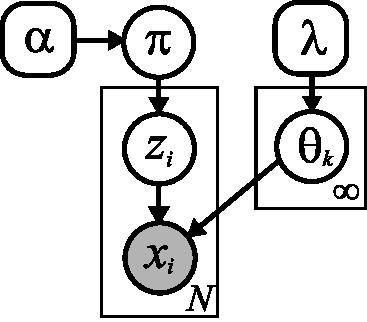
\includegraphics[width=20mm]{sudderth-infiniteMixIndGraph}}
\subfigure[]{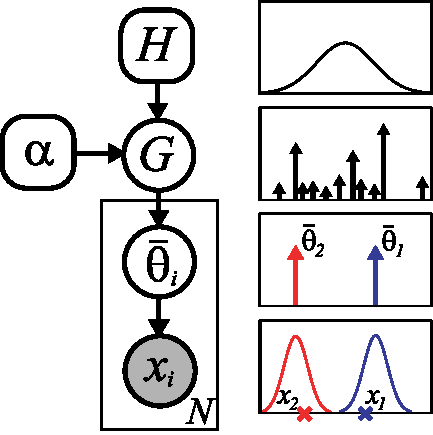
\includegraphics[width=20mm]{sudderth-infiniteMixDistGraphExampleData}}
%\caption{}
\end{figure}
\begin{itemize}
    \item The DP is not particularly useful as a model for data directly, since data vectors rarely repeat exactly.
    \item Useful as a prior for the parameters to generate data.
    \item Define $G \sim \text{DP}(\alpha,H)$. Equivalently, we can write the model
    \begin{equation*}\small
        \begin{split}
            \bm{\pi} & \sim \text{GEM}(\alpha), \quad
            z_i \sim  \bm{\pi}\\
            %G = & \sum_{k= 1}^K \pi_k\delta_{\theta_k} (\theta)\\
            \bm{\theta}_k & \sim H(\lambda)\\
            \bm{x}_i & \sim F(\bm{\theta}_{z_i})
        \end{split}    
    \end{equation*}

\end{itemize}    
\end{frame}

\begin{frame}{Gaussian mixture model}
\begin{equation*}
    \begin{split}
        \bm{\pi} & \sim \text{GEM}(\alpha), \quad
            z_i \sim  \bm{\pi}\\
        G & = \sum_{k=1}^K \pi_k\delta_{\bm{\theta}_k} (\bm{\theta}) = \text{DP}(\alpha,N(\bm{\mu}_0,\bm{\Sigma}_0))\\
        \bm{\mu}_i & \sim G\\
        \bm{x}_i & \sim N(\bm{\mu}_i,\bm{\Sigma})
    \end{split}        
\end{equation*}
    
\end{frame}

\begin{frame}{Fitting a DP mixture modeling}
\begin{itemize}
    \item Fit a DPMM by modifying the collapsed Gibbs sampler.
    \begin{equation*}\small
        p(z_i = k|\bm{z}_{-i}, \bm{x}, \alpha, \bm{\lambda}) \propto p(z_i = k|\bm{z}_{-i}, \alpha)p(\bm{x}_i|\bm{x}_{-i}, z=k, \bm{z}_{-i}, \bm{\lambda})
    \end{equation*}
    \item The first term is given by
    \begin{equation*}\small
        p(\bm{z}_i|\bm{z}_{-i},\bm{\alpha})= \frac{\mathbb{I}}{\alpha+N-1} (\alpha \mathbb{I}(z=k^*)+ \sum_{k=1}^K N_{k,-i} \mathbb{I} (z=k) )
    \end{equation*}
    \item If $z_i = k$, then $\bm{x}_i$ is conditionally independent of all the data points except those assigned to cluster $k$. Hence 
    \begin{equation*}
        p(\bm{x}_i|\bm{x}_{-i}, \bm{z}_{-i}, z_i = k, \bm{\lambda}) = p(\bm{x}_i|\bm{x}_{-i,k}, \bm{\lambda}) = \frac{p(\bm{x}_i,\bm{x}_{-i,k}|\bm{\lambda})}{p(\bm{x}_{-i,k}|\bm{\lambda})}
    \end{equation*}
    where
    \begin{equation*}\small
        p(\bm{x}_i,\bm{x}_{-i,k}|\bm{\lambda}) = \int p(\bm{x}_i|\bm{\theta}_k) \left[\prod_{j \neq i, z_j = k} p(\bm{x}_j|\bm{\theta}_k)\right]H(\bm{\theta}_k|\bm{\lambda})d\bm{\theta} _k    
    \end{equation*}
\end{itemize}    
\end{frame}

\begin{frame}{Fitting a DP mixture modeling(cont'd)}
\begin{itemize}
    \item If $z_i = k^*$, corresponding to a new cluster, we have
    \begin{equation*}\small
        p(\bm{x}_i|\bm{x}_{-i}, \bm{z}_{-i}, z_i = k^*,\bm{\lambda}) = p(\bm{x}_i|\bm{\lambda}) = \int p(\bm{x}_i|\bm{\theta})H(\bm{\theta}|\bm{\lambda})d\bm{\theta}
    \end{equation*}
\end{itemize}    

\noindent\rule[-5pt]{\textwidth}{0.4pt}
{\footnotesize
\begin{tabbing}
    {\bf Initialize} \\*[\smallskipamount]
    {\bf for} each $i=1:N$ in random order {\bf do}\\
    \= Remove $\bm{x}_i$'s sufficient statistics from old cluster $z_i$. \\
        \qquad {\bf for} each $k=1:K$ {\bf do}\\
        \qquad \= Compute $p_k(\bm{x}_i) = p(\bm{x}_i|\bm{x}_{-i}(k))$.\\
        \> Set $N_{k,-i} = \text{dim}(\bm{x}_{-i}(k))$.\\
        \> Compute $p(z_i = k|z_{-i, D}) = \frac{N_{k,-i}}{\alpha+N-1}$. \\*[\smallskipamount]
    \= Compute $p_*(\bm{x}_i) = p(\bm{x}_i|\bm{\lambda})$. \\
    \> Compute $p(z_i = ∗|\bm{z}_{-i}, D) = \frac{\alpha}{\alpha+N-1}$.\\
    \> Normalize $p(z_i |.)$.\\
    \> Sample $z_i \sim p(z_i |.)$.\\
    \> Add $\bm{x}_i$'s sufficient statistics to new cluster $z_i$.\\
    \> If any cluster is empty, remove it and decrease $K$.
\end{tabbing}}
\noindent\rule[10pt]{\textwidth}{0.4pt}
\end{frame}

\section{Spectral clustering}
\begin{frame}{Data Clustering}
\begin{itemize}
    \item Two different criteria
    \begin{itemize}
        \item Compactness, e.g., k-means, mixture models
        \item Connectivity, e.g., spectral clustering
    \end{itemize}
\end{itemize}  

\begin{figure}[h]
\centering
\subfigure[]{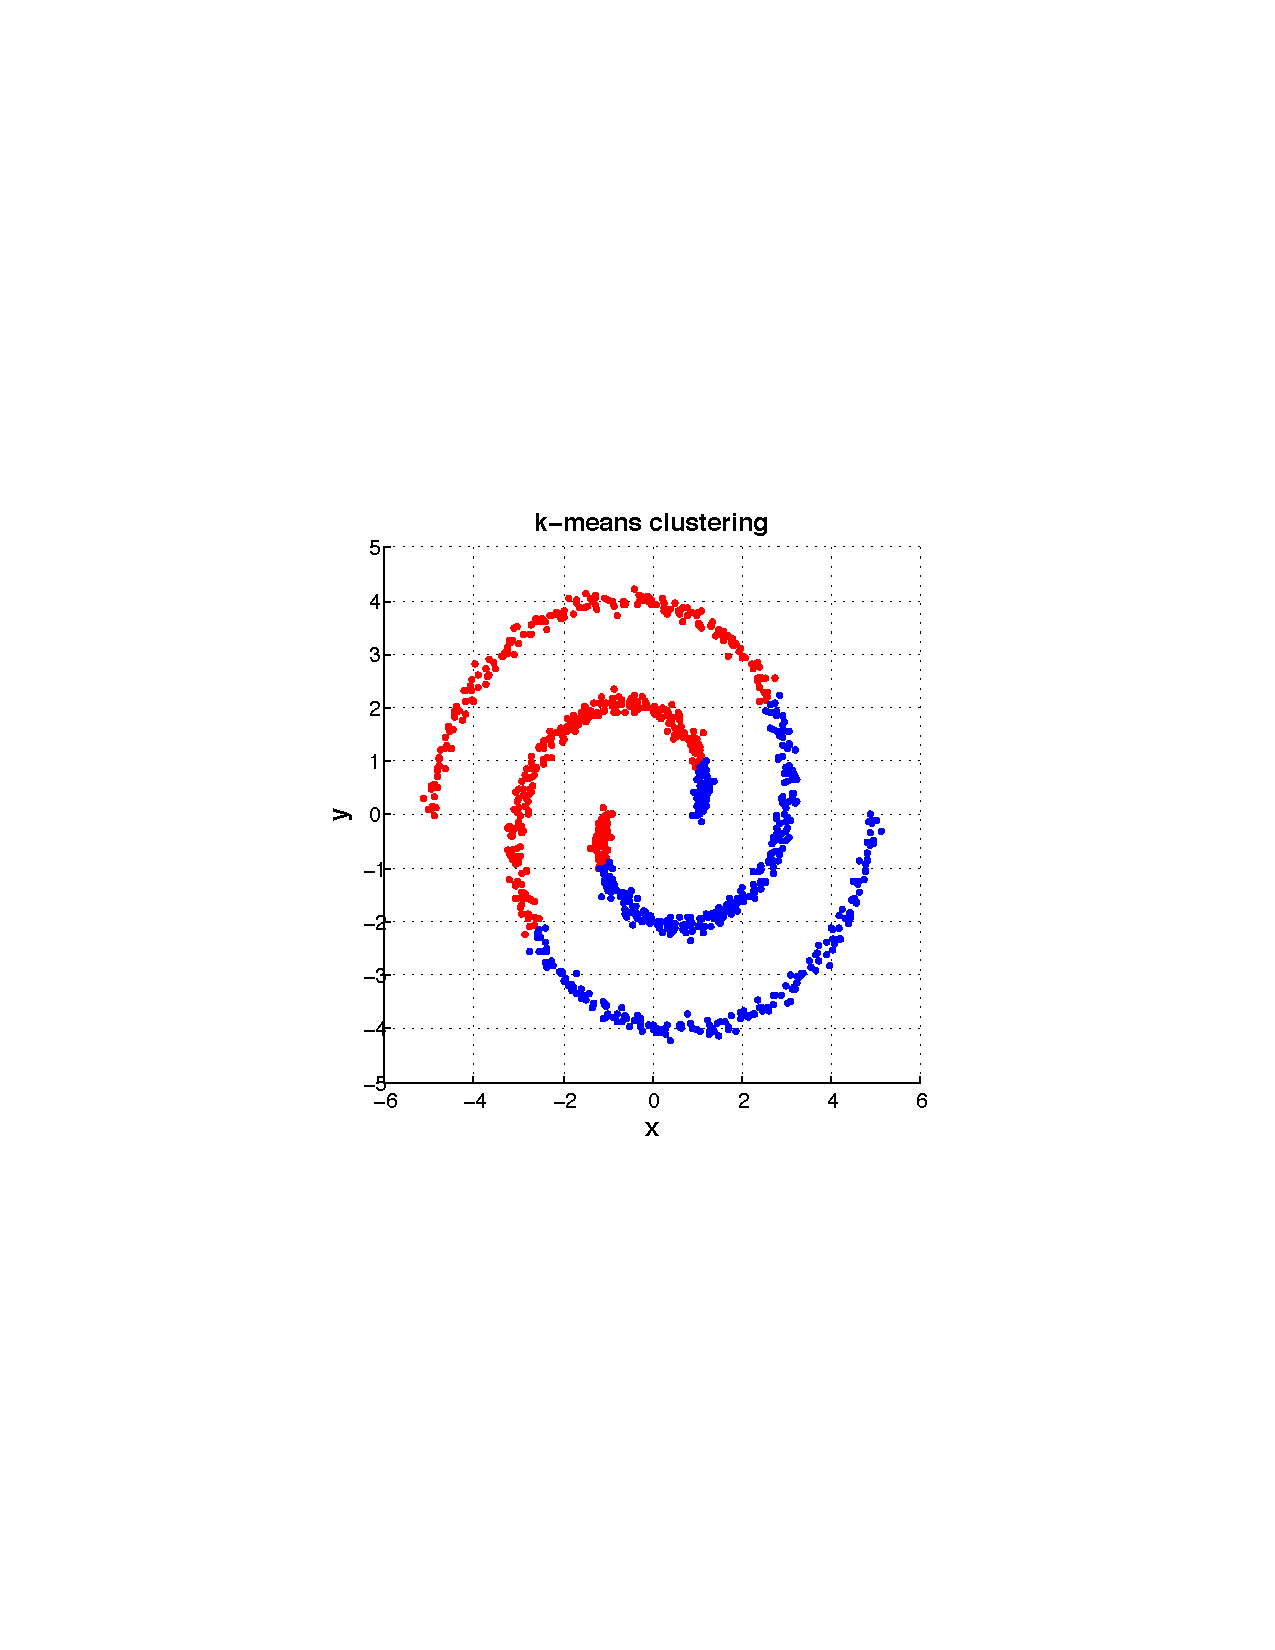
\includegraphics[width=20mm]{spiral-kmeans}}
\subfigure[]{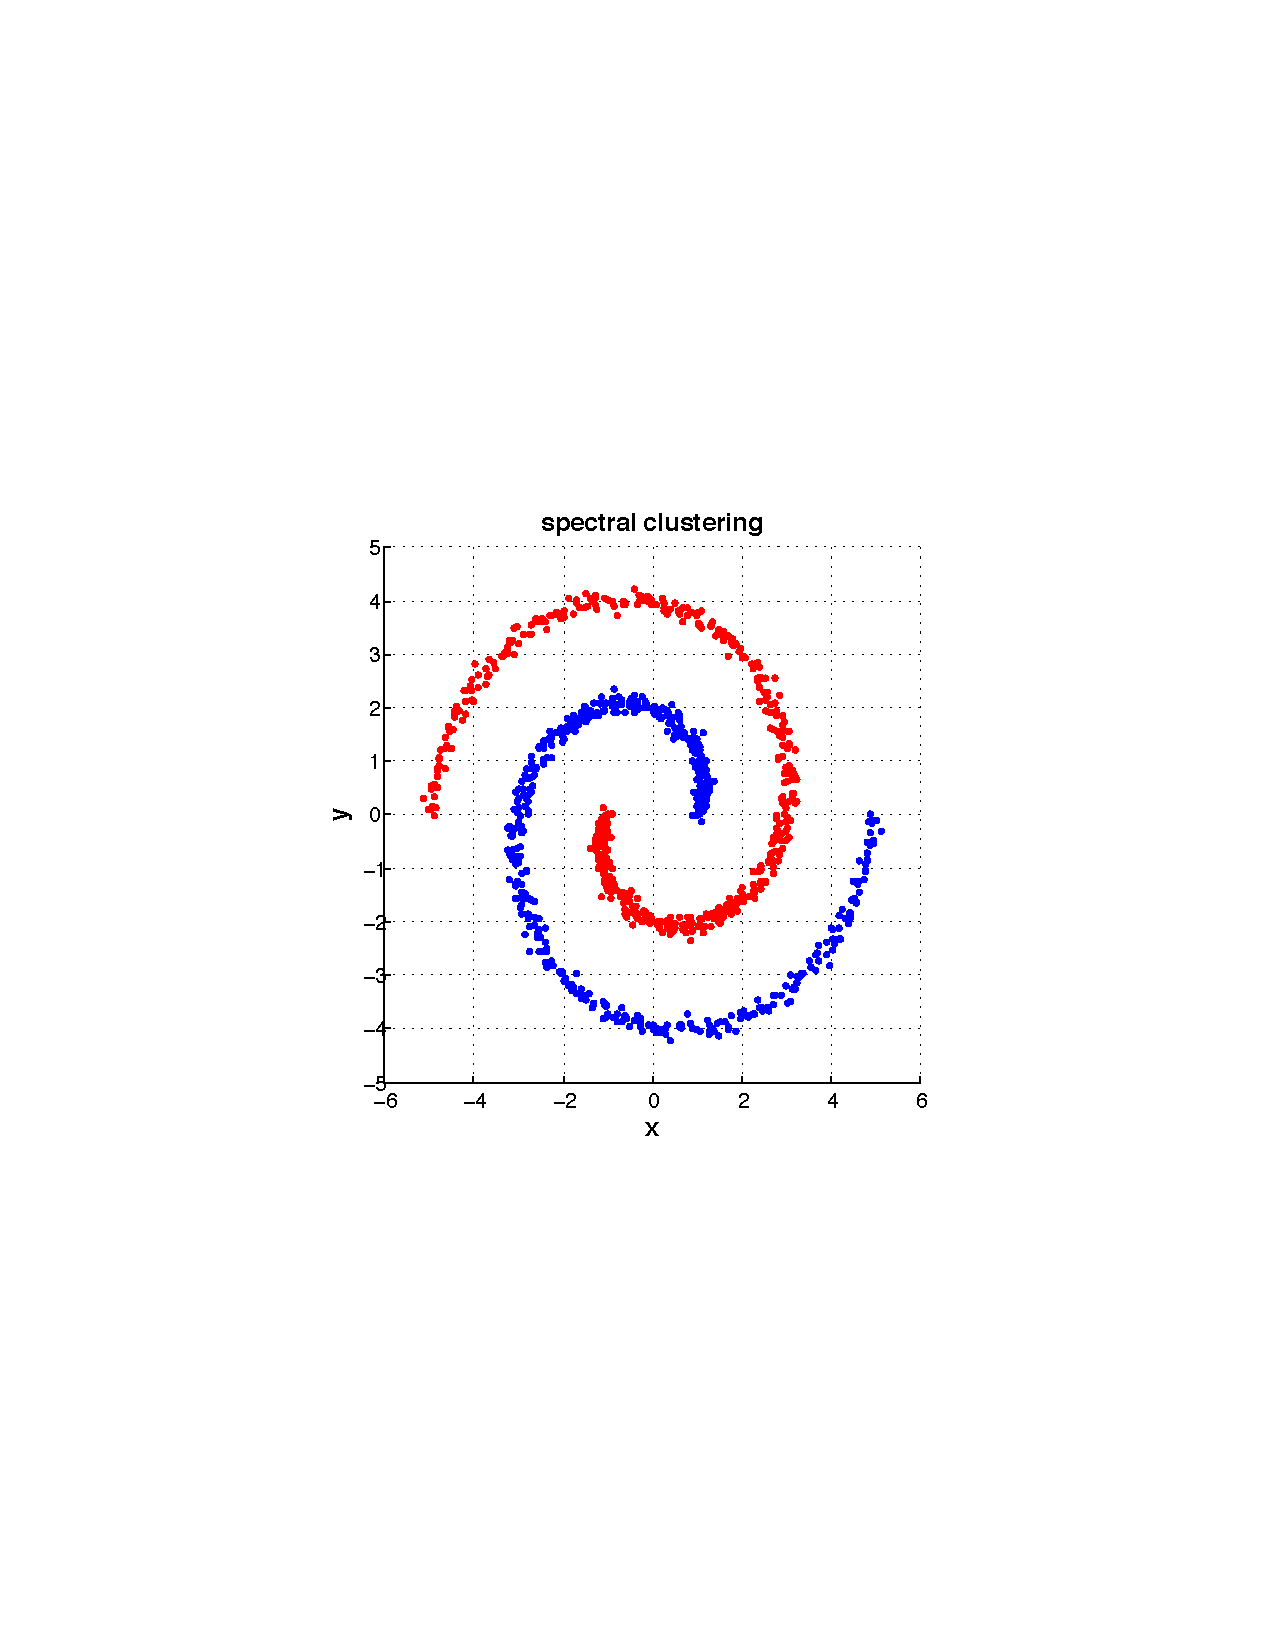
\includegraphics[width=20mm]{spiral-spectral}}
\caption{Clustering data consisting of 2 spirals. (a) K-means. (b) Spectral clustering. Figure generated by \texttt{SpectralClusteringDemo}, written by Wei-Lwun Lu.}
\end{figure}
\end{frame}

\begin{frame}{Weighted Graph Partitioning}
\begin{itemize}
    \item Some graph terminology
    \begin{itemize}
        \item Objects  (e.g.,pixels,data points) $ i \in I$ = vertices of graph $G$.
        \item Edges ($ij$) = pixel pairs with $W_{ij} > 0$.
        \item Similarity matrix $\bm{W} = [ W_{ij} ]$.
        \item Degree
        \begin{equation*}
            \begin{split}
                d_i = &  \sum_{j \in G} W_{ij}\\
                d_A = & \sum_{i \in A} d_i \quad \text{degree of} \quad A \subseteq G
            \end{split}
        \end{equation*}
        \item $\text{Assoc}(A, B) = \sum_{i \in A}\sum_{j \in B}W_{ij}$
    \end{itemize}
\end{itemize}  
\end{frame}

\begin{frame}{Cuts in a Graph}
\begin{itemize}
    \item Edge cut = set of edges whose removal makes a graph disconnected.
    \item Weight of a cut:
    \begin{equation*}
        \text{cut}(A, B) = \sum_{i \in A}\sum_{j \in B}W_{ij} = \text{Assoc}(A, B) 
    \end{equation*}
    \item Normalized Cut criteria: minimum $\text{cut}(A, \bar{A})$
    \begin{equation*}
        \text{Ncut}(A, \bar{A}) = \frac{\text{cut}(A, \bar{A})}{d_A} + \frac{\text{cut}(A, \bar{A})}{d_{\bar{A}}} 
    \end{equation*}
\end{itemize}  
\end{frame}

\begin{frame}{Graph-based Clustering}
\begin{itemize}
    \item Affinity matrix: $\bm{W} = [ W_{ij} ]$.
    \item Degree matrix: $\bm{D} = \text{diag}(d_i)$.
    \item Laplacian matrix: $\bm{L} = \bm{D} - \bm{W}$.
    \item (Bipartite) partition vector: 
    \begin{equation*}
        \bm{x} = [x_1,\ldots,x_n] = [1,1,\ldots,-1,\ldots,-1]
    \end{equation*}
\end{itemize}  
\end{frame}

\begin{frame}{Clustering via Optimizing Normalized Cut}
\begin{itemize}
    \item The normalized cut:
    \begin{equation*}
        \text{Ncut}(A, B) = \frac{\text{cut}(A, B)}{d_A} +  \frac{\text{cut}(A, B)}{d_B}
    \end{equation*}
    
    \item Transform Ncut equation to a matrix form (Shi \& Malik 2000):
    \begin{equation*}
    \min_x \text{Ncut} (x) =  \min_y \frac{y^T(\bm{D}-\bm{W})y}{y^T\bm{D}y}
    \end{equation*}
    
    \begin{equation*}
        \begin{split}
            \text{subject to: } & y \in \{1,-b\}^n \\ & y^T\bm{D}\bm{1} = 0 
        \end{split}
    \end{equation*}
\end{itemize}  
\end{frame}

\begin{frame}
\begin{itemize}
    \item Relax the continuous domain by solving generalized eigenvalue system:
    \begin{equation*}
         \min_y y^T(\bm{D}-\bm{W})y, \quad \text{s.t.} \quad y^T\bm{D}y = \bm{1}
    \end{equation*}
    \begin{itemize}
        \item Which gives: 
        \begin{equation*}
            (\bm{D}-\bm{W})y = \lambda \bm{D}y
        \end{equation*}
        \item Note that $(\bm{D}-\bm{W})\bm{1} = 0$ so, the first eigenvector is $y_0=1$ with eigenvalue $0$.
        \item The second smallest eigenvector is the real valued solution to this problem.
    \end{itemize}
\end{itemize}
    
\end{frame}
\begin{frame}{Algorithm}
\begin{itemize}
    \item Define a similarity function between 2 nodes. i.e.
    \begin{equation*}
        W_{i,j} = \exp(-\frac{\|X_{(i)} - X_{(j)}\|_2^2}{\sigma_X^2})
    \end{equation*}
    \item Compute affinity matrix ($\bm{W}$) and degree matrix ($\bm{D}$).
    \item Solve
    \begin{equation*}
        (\bm{D}-\bm{W})y = \lambda \bm{D}y
    \end{equation*}
    \begin{itemize}
        \item Do singular value decomposition (SVD) of the graph Laplacian $\bm{L} = \bm{D} - \bm{W}$.
        \begin{equation*}
            \bm{L} = \bm{V}^T \bm{\Lambda} \bm{V} 	\Rightarrow y^*
        \end{equation*}
    \end{itemize}
    \item Use the eigenvector with the second smallest eigenvalue, bipartition the graph
    \begin{itemize}
        \item For each threshold $k$,
        \begin{equation*}
            \begin{split}
                A_k & =\{i | y_i \text{ among } k \text{ largest element of } y^*\}\\
                B_k & =\{i | y_i \text{ among } n-k \text{ smallest element of } y^*\}
            \end{split}
        \end{equation*}
        \item Compute $\text{Ncut}(A_k,B_k)$
        \item Output: $k^* = \argmax\text{Ncut}(A_k,B_k)$, $A_{k^*},B_{k^*}$
    \end{itemize}  
\end{itemize}  
\end{frame}

\end{document}
